% vi:ft=tex
\documentclass{standalone}

\usepackage{tikz}
\usepackage{verbatim}

\usetikzlibrary{arrows}
\usetikzlibrary{calc}
\usetikzlibrary{shapes}

\begin{document}

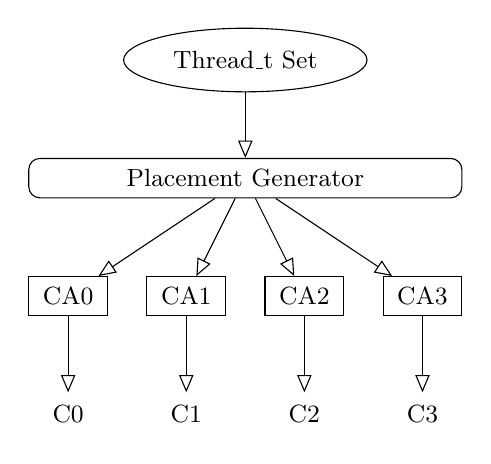
\begin{tikzpicture}[node distance = 1.5cm]

  % Colors
  % Styles
  \tikzstyle{defaultRec} = [font=\small, text centered, inner sep = 1pt,
    draw=black, shape=rectangle, fill=white, anchor=center, minimum height = .5cm];
  \tikzstyle{coreAcc} = [defaultRec, minimum width=1cm];
  \tikzstyle{pGen} = [defaultRec, rounded corners];

  \tikzstyle{defaultCirc} = [font=\small, text centered, inner sep = 1pt,
    draw=none, shape=circle];
  \tikzstyle{core} = [defaultCirc];
  \tikzstyle{threadSet} = [defaultCirc, shape=ellipse, draw=black, inner sep =
  5pt];

  \tikzstyle{arrow} = [-open triangle 45, thin, black];

  % Variables
  \newcommand\Ymax{3};
  \newcommand\Xmax{7};
  \newcommand\fstLvl{1};
  \newcommand\sndLvl{2};

  % Drawing
  \node(c0) [core] {C0};
  \node(c1) [core, right of=c0] {C1};
  \node(c2) [core, right of=c1] {C2};
  \node(c3) [core, right of=c2] {C3};

  \node(ca0) [coreAcc, above of=c0] {CA0};
  \node(ca1) [coreAcc, above of=c1] {CA1};
  \node(ca2) [coreAcc, above of=c2] {CA2};
  \node(ca3) [coreAcc, above of=c3] {CA3};

  \draw[transparent] (ca0.west) -- ++(0,1.5cm) coordinate(help) [at end];

  \node(pGen) [pGen, right of=help, anchor=west, node distance=0, minimum width=5.5cm] {Placement Generator};

  \node(ts) [threadSet, above of=pGen] {Thread\_t Set};

  \draw[arrow] (ts) to (pGen);
  \draw[arrow] (pGen) to (ca0);
  \draw[arrow] (pGen) to (ca1);
  \draw[arrow] (pGen) to (ca2);
  \draw[arrow] (pGen) to (ca3);

  \draw[arrow] (ca0) to (c0);
  \draw[arrow] (ca1) to (c1);
  \draw[arrow] (ca2) to (c2);
  \draw[arrow] (ca3) to (c3);

%  \node [defaultRec, draw=none, left of=ca0, node distance=1cm, anchor=east,
%  black!50]
%    {handles SMT};
\end{tikzpicture}

\end{document}
